\subsection{Polarized Proton Collisions}

``A cross section is written in factorized form as a convolution of parton distribution functions and fragmentation functions with a partonic subprocess cross section''

Assumptions:
\begin{itemize}
  \item Cross section can be written in factorized form
  \item Universality of parton distribution functions
  \item Universality of fragmentation functions
  \item partonic cross section calculable in perturbative QCD
\end{itemize}

First bullet point relies on the next 3, of course.

\begin{equation}
  A_{LL} = \frac{\sum_{f_1,f_2,f}~\Delta f_1 \otimes \Delta f_2 \otimes \sigma^{f_1 f_2 \rightarrow f X'} \hat a_{LL}^{f_1 f_2 \rightarrow f X'} \otimes D_f}{\sum_{f_1,f_2,f}~f_1 \otimes f_2 \otimes \sigma^{f_1 f_2 \rightarrow f X'} \otimes D_f} 
\end{equation}

\begin{equation}
  \hat a_{LL}^{f_1 f_2 \rightarrow f X'} = \frac{\Delta \sigma^{f_1 f_2 \rightarrow f X'}}{\sigma^{f_1 f_2 \rightarrow f X'}}
\end{equation}

\begin{figure}\begin{center}
  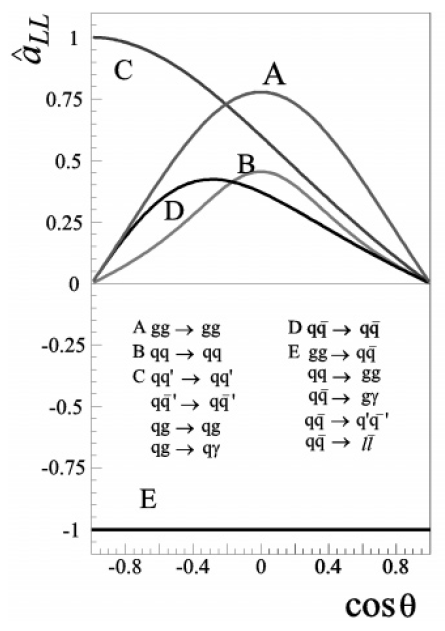
\includegraphics[width=0.5\textwidth]{figures/partonic_asymmetry}
  \caption{\cite{Bunce:2000uv}}
\end{center}\end{figure}
